\section{Introduction}
\label{sec:intro}
%SSO的特点
%SSO的现状

%SSO系统的安全问题,需要保护identity proof的完整性,机密性,绑定性
%完整性:使用公开的为受保护的信息作为identity proof
%机密性:保证由IdP发送给对应的RP,并且传输过程中通道、user agent都是受到保护的
%绑定性:identity proof一定要与对应的RP实现绑定
%SPRESSO中关于impersonation和identity injection的描述。 Authentication is the most fundamental security property of an SSO system. That is, i) an adversary should not be able to log in to an RP, and hence, use the service of the RP, as an honest user, and ii) an adversary should not be able to log in the browser of an honest user under an adversary’s identity (identity injection).
%这段描述两个事情:1.secure authentication 就是能防住impersonation和identity injection。 然而,现在有很多攻击使得这两个无法得到保证。经过分析主要是这三个方面的原因:1)RP接受了未被完整性保护的内容;2)未绑定;3)泄露。
%binding 原文描述 ChenPCTKT14 CCS14 Friendcaster(Friendcaster是一款Facebook的第三方应用,比官方版的功能更加全面) blindly accepting an access token received from a user's device then using this token to exchange for the user's Facebook ID. A malicious application could obtain a legitimate access token from a user, then use this access token to log into Friendcaster as the user. cause they thought Facebook's access tokens were bound to relying parties and checked with every API call: \From Facebook's perspective, the API calls wouldn't appear to be originating from Friendcaster, but the attacker's own app."
%完整性原文描述 IEEE S&P2012~\cite{WangCW12}关于Google问题描述we found that the RPs of Google ID SSO often assume that message fields they require Google to sign would always be signed, which turns out to be a serious misunderstanding (Section 4.1). These problems make us believe that a complete answer to our question can only be found by analyzing SSO schemes on real websites.

% Move to section III
%The primary goal of SSO services is to implement secure user authentication~\cite{SPRESSO}, i.e., to ensure that an honest user can always log in to an honest RP under the correct account. To achieve this, an identity proof generated by the IdP should explicitly specify the authenticated user (i.e., \emph{user identification}) and the RP to which the user attempts to log in (i.e., \emph{receiver designation}). The identify proof should be received only by that RP and user but not by any other entities (i.e., \emph{confidentiality}) and verified by the receiver (i.e., \emph{integrity}). However, various attacks exploit vulnerabilities in different SSO systems to break at least one of these requirements~\cite{ChenPCTKT14, FettKS16,WangCW12,ZhouE14,WangZLG16,YangLLZH16,SomorovskyMSKJ12,MohsenS16}, where the adversaries attempt to either impersonate the victim user at an honest RP or %manipulate the victim user's browser to log in to honest RPs under the adversary's identity. %(i.e., identity injection). For example, Friendcaster was found to accept any received identity proof~\cite{ExplicatingSDK,ChenPCTKT14} (i.e., a violation of receiver designation) so that a malicious RP could log in to Friendcaster as the victim user by replaying the identity proof received from the user to Friendcaster~\cite{MohsenS16}. \cite{WangCW12} reported that some RPs of Google ID SSO accepted user attributes that were not tied to the identity proof (i.e., a potential violation of integrity). As a result, a malicious user could insert arbitrary attributes (e.g., an email address) into the identity proof to impersonate another user at the RP.


%SSO 引入新的隐私问题
%IdP知道用户登录哪个RP
%RP之间可以合谋知道同一个用户登录哪些RP
Single sign-on (SSO) systems such as OpenID Connect (OIDC)~\cite{OpenIDConnect}, OAuth~\cite{rfc6749} and SAML~\cite{SAML} have been widely deployed in today's Internet for identity management and authentication. With SSO, a user can log in to a website, referred to as the relying party (RP), using her account registered at another website, known as the identity provider (IdP). An RP delegates user authentication to a trusted IdP, who then generates identity proofs for the users visiting the RP. Therefore, the user needs to remember only one credential at the IdP, instead of maintaining multiple credentials for different RPs.
%Moreover, SSO shifts the burden of user authentication from RPs to IdPs and reduces security risks and costs at RPs.

%SSO has been widely integrated into many application services. For example, 80\% of the Alexa Top-100 websites and 6.3\% of the Alexa Top-1M websites support SSO~\cite{GhasemisharifRC18}. Meanwhile, many email and social network providers (such as Google, Facebook, Twitter, etc.) are serving the IdP roles.

However, SSO systems have been continuously found vulnerable and insecure~\cite{WangCW12,ccsSunB12,SomorovskyMSKJ12,ArmandoCCCPS13,DiscoveringJCS,dimvaLiM16,WangZLG16,MainkaMS16, MainkaMSW17,YangLCZ18}. Besides, the adoption of SSO raises public concern about user privacy~\cite{maler2008venn,NIST2017draft,BrowserID,SPRESSO}, in the fear that an adversary may be able to track to which RP(s) the user has logged in. {\em Unfortunately, almost all the existing SSO protocols leak user privacy in different ways.} Take a widely used SSO protocol, OIDC, as an example. As shown in Fig.~\ref{fig:OpenID}, the login process starts when a user sends a login request to the RP, % (Step 1),
who then constructs a request for identity proof with its identity and redirects the request to the IdP. % (Step 2).
After authenticating the user, the IdP generates an identity proof with the identities of both the user and RP, %in Step 4,
which is returned to the user and forwarded to the RP. %in Step 5.
Finally, the RP verifies the identity proof to decide if the user is allowed to log in. In such login instances, by design, an IdP can always see when and where a user attempts to log in, to generate the identity proof. As a result, a curious IdP can easily track the RPs that a target user has visited over time. This data can be further analyzed to profile users' online activities, as in other web tracking attacks. So, we call this privacy attack \textbf{\em IdP-based login tracing}, which has also been reported by previous research~\cite{BrowserID,SPRESSO}. Similarly, by design, the RPs can learn users' identities from the received identify proofs. If the IdP uses a unique or related user identifier(s) to generate identity proofs for her to access different RPs~\cite{Google, FirefoxAccount}, curious RPs can collude to link the login requests, associate her attributes across multiple RPs, and track her online activities~\cite{maler2008venn}. We denote this privacy risk as \textbf{\em RP-based identity linkage}.

As SSO becomes a popular safeguard for various privacy-sensitive web services, the privacy concern is considered more prominent and severe than it was in the past. Recently, many IdPs have taken user privacy in SSO into serious consideration and offered new protection against RP-based identity linkage. For example, Figure~\ref{fig:wechat} shows the IdP service provided by WeChat, one of the most popular instant messaging applications in China. It allows a user to create new accounts with new profile attributes to log in to different RPs. Similarly, IdPs such as NORDIC APIS and CURITY suggest adopting pairwise pseudonymous identifier (PPID) in SSO~\cite{Nordic, Curity}, and Active Directory Federation Services~\cite{MS} and Oracle Access Management~\cite{Oracle} support the use of PPID.

However, these efforts cannot protect users from IdP-based login tracing. While privacy-savvy users may provide few personal information to web applications to avoid user tracking or profiling, the use of popular SSO services such as Google Account opens a door for IdPs and application providers to recover users' online traces and profiles, which makes users' privacy protection effort in vain. Several large IdPs, especially the social IdPs, are known to be interested in collecting users' online behavioral data for various purposes (e.g., Screenwise Meter~\cite{googlenews} and Onavo~\cite{Onavo}). Serving the IdP role makes it possible for them to collect such information. Meanwhile, service providers hosting multiple web applications take an advantaged position to correlate users' multiple logins at different RPs through internal information integration. Finally, privacy-preserving record linkage~\cite{agrawal2003information} and private set intersection~\cite{de2010practical} technologies allow multiple RPs to share data without violating the privacy policies, which pave the path for cross-organizational RP-based identity linkage.

\begin{figure}[t]
  \centering
  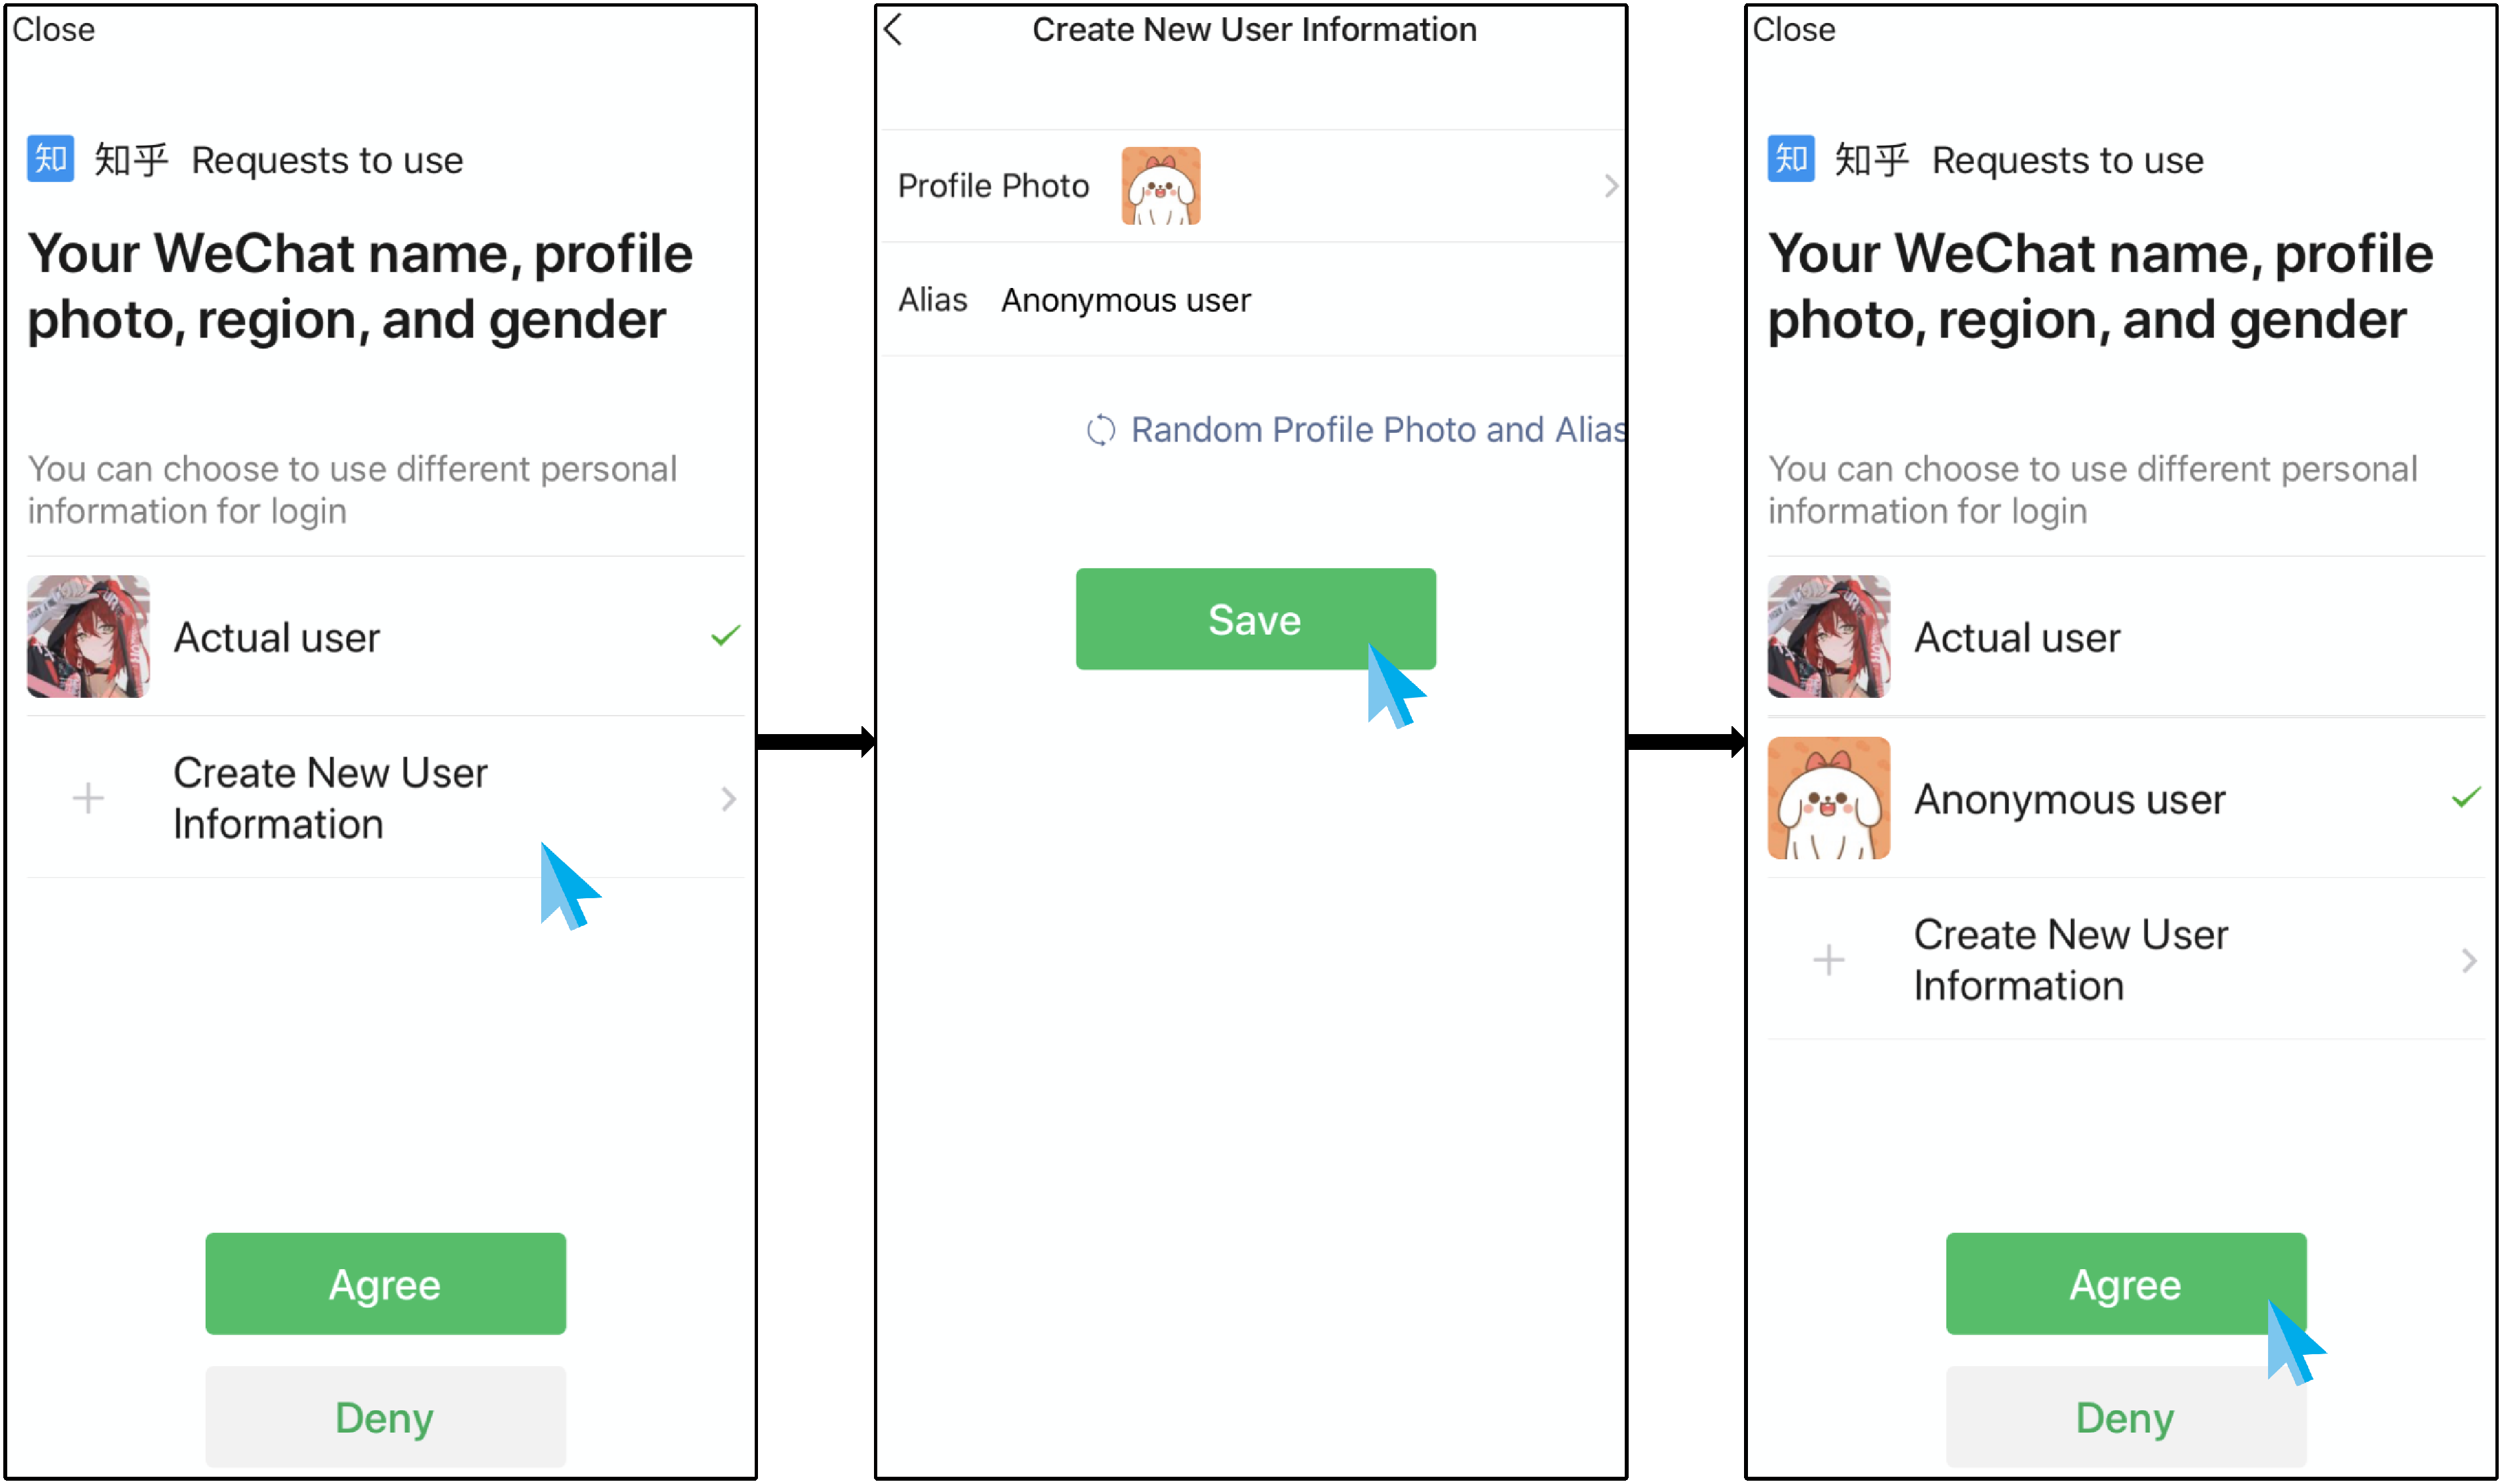
\includegraphics[width=0.9\linewidth]{fig/wechat.pdf}
  \caption{Anonymous SSO login in WeChat.}
  \label{fig:wechat}
  \vspace{-5mm}
\end{figure}

%also raises privacy concerns regarding online user tracking and profiling.
%Imagine that, a user concerning her privacy would avoid to leave her full sensitive information at an application. The user may use multiple web applications and only leave parts of her sensitive messages at each applications, for example, using  real name on social website, the address on shopping website and the phone number on Telecom website. And she would try not to leave any linkable message to avoid applications combining her informations, for example, if she leave the email on each applications, they can combine the parts of informations through the email. However,  the privacy leaks in SSO systems make her effort in vain. As long as a user employs the SSO system, such as Google Account, to log in to these applications, the applications providers and Google can combine your informations based on the SSO account.

%google and facebook的负面新闻
%1. service provider(如DNS)知道你访问了,可以带来很多问题。但是还是不同的,DNS里profile需要评估的是two behavior vectors的similarities,而IdP中都不需要,因为IdP能够区分two behavior vectors 是否来自相同节点。

Several solutions have been proposed to protect user privacy in SSO login~\cite{maler2008venn,NIST2017draft,BrowserID,SPRESSO}. However, to the best of our knowledge, {\em none of them provides a comprehensive protection against IdP-based login tracing and RP-based identity linkage at the same time} (we provide a brief review of existing solutions and their limitations in Section~\ref{subsec-solutions}). Moreover, the techniques proposed so far to defend each of the two attacks cannot be directly integrated, since they require modifications to the SSO flows that are essentially conflicting and cannot occur simultaneously. This requires a non-trivial re-design of the SSO system to defend against both attacks,
%IdP-based login tracing and RP-based identity linkage
while providing a secure and compatible SSO service.

In this paper, we are among the first to conceptualize the privacy problem in SSO as {\em an identifier transformation problem} and explain the reasons that limit existing solutions from fully protecting user privacy against curious IdPs and collusive RPs. Based on our analysis, we propose an Unlinkable Privacy-PREserving Single Sign-On (UPPRESSO) system for comprehensive protection against both privacy attacks. In particular, UPPRESSO designs three one-way identifier-transformation functions based on the elliptic curve cryptography. The first two convert the identities of the user and RP into privacy-preserving pseudo-identifiers using a randomly chosen trapdoor $T$. This prevents IdP-based login tracing by hiding the RPs' identities from the IdP and RP-based identity linkage by hiding the user's identity from the RPs. Meanwhile, an RP can link multiple login sessions of the same user by converting her different pseudo-identifiers to an invariant user account using a special identifier-transformation function and the trapdoor $T$, without knowing the user's real identity. Finally, we formally prove that the accounts of the same user at different RPs are independent and cannot be correlated by collusive RPs (in Section~\ref{sec:privacy}).
%UPPRESSO designs three one-way identifier-transformation functions based on elliptic curve cryptography. Using the one-way trapdoor function $\mathcal{F}_{ID_{RP} \mapsto PID_{RP}}(ID_{RP}, T)$, the RP converts its identity $ID_{RP}$ into a privacy-preserving pseudo-identifier $PID_{RP}$ based on a randomly selected trapdoor $T$. Similarly, the IdP uses the one-way function  $\mathcal{F}_{ID_{U} \mapsto PID_{U}}(ID_U, PID_{RP})$ to generate a privacy-preserving pseudo-identifier $PID_U$ for the user based on her identity $ID_U$ and $PID_{RP}$. Finally, using a special identifier-transformation function $\mathcal{F}_{PID_{U} \mapsto Account}(PID_U, PID_{RP}, T)$, the RP is able to map all the different privacy-preserving pseudo-identifiers of a user, which are created in her different login sessions to that RP, to a same $Account$ that identifies the user to the RP. The three identifier-transformation functions work cooperatively to ensure: (\emph{a}) when a user logs in to an RP multiple times, the RP can always map $PID_U$s to a unique $Account$ without knowing the user's identity $ID_U$; moreover, when a user logs in to multiple RPs, (\emph{b}) a curious IdP learns nothing about the identities of these RPs from $PID_{RP}$s, and (\emph{c}) collusive RPs cannot link $PID_U$s to a particular user %or associate them together, (\emph{d}) nor correlate $Account$s of a same user at different RPs.
We summarize our contributions as follows.
%我们的贡献
%提出协议
%考虑能否根据模型进行分析
%实现原型系统
%The main contributions of UPPRESSO are as follows:
\begin{itemize}
\vspace{-\topsep}
\item We formalize the SSO privacy problems as an identifier-transformation problem and analyze the limitations of existing privacy solutions for SSO.
\vspace{-\topsep}
\item We propose a comprehensive solution to hide the users' login traces from curious IdPs and collusive RPs. To the best of our knowledge, UPPRESSO is the first SSO system that secures SSO services against IdP-based login tracing and RP-based identity linkage.
\vspace{-\topsep}
\item We formally prove the privacy of UPPRESSO based on the DDH assumption~\cite{GoldwasserK16} and the security of UPPRESSO based on a formal model of the web infrastructure. Our results show that UPPRESSO provides expected and satisfying security and privacy protection to SSO.
%provide the reduction from UPPRESSO scheme to DDH Assumption proving that it is protected from IdP-based login tracing and RP-based identity linkage,
%and analyze the security of UPPRESSO based on a formal model of the web infrastructure and formally prove that it provides satisfying security properties.
\vspace{-\topsep}
\item UPPRESSO is compatible with existing SSO systems, since it requires only small modifications to support new identifier-transformation functions. We implement a prototype of UPPRESSO based on an open-source implementation of OIDC, which leverages HTML 5 features in the implementation and thus can be used across platforms (e.g., PCs, smartphones, and other devices). %Unlike  BrowserID and SPRESSO,  does not require non-trivial re-designs of SSO services, which makes it more .
\vspace{-\topsep}
\item We compare the performance of our UPPRESSO prototype with the state-of-the-art SSO systems (i.e., OIDC~\cite{OpenIDConnect} and SPRESSO~\cite{SPRESSO}) and demonstrate its efficiency.
\end{itemize}
\vspace{-\topsep}
%文章结构
The rest of the paper is organized as follows. We introduce the background in Section~\ref{sec:background}, the privacy problem and our design ideas in Section~\ref{sec:challenge}, and the threat model in Section~\ref{sec:assumptionandthreatmodel}. Section \ref{sec:UPPRESSO} describes the detailed design of UPPRESSO based on identifier transformation, followed by a formal analysis of the privacy and security in Sections~\ref{sec:privacy} and ~\ref{sec:formal}. We explain the implementation specifics and experimental evaluation in Section~\ref{sec:implementation}, discuss the extensions and related works in Sections~\ref{sec:discussion} and~\ref{sec:related}, and conclude our work in Section~\ref{sec:conclusion}.

%   © 2021 GitHub, Inc.
%    Terms
%    Privacy
%    Security
%    Status
%    Docs
